\documentclass[english,14pt]{beamer}
\usetheme{EastLansing}
\usecolortheme{spruce}

\usepackage{xcolor}
\usepackage{listings}
\usepackage{courier}
\usepackage{graphicx}
\usepackage{amsmath}
\usepackage{algorithm2e}
\usepackage{multicol}
\usepackage{hyperref}

% http://mirrors.ibiblio.org/CTAN/macros/latex/contrib/datetime2/datetime2.pdf
\usepackage{babel}
\usepackage[useregional]{datetime2}

% https://tex.stackexchange.com/questions/42619/x-mark-to-match-checkmark
\usepackage{pifont}% http://ctan.org/pkg/pifont

%% https://stackoverflow.com/questions/1435837/how-to-remove-footers-of-latex-beamer-templates
%%gets rid of bottom navigation bars
%\setbeamertemplate{footline}[page number]
%
%gets rid of navigation symbols
\setbeamertemplate{navigation symbols}{}


\usefonttheme[onlymath]{serif}

\definecolor{mGreen}{rgb}{0,0.6,0}
\definecolor{mGray}{rgb}{0.5,0.5,0.5}
\definecolor{mPurple}{rgb}{0.8,0,0.82}
\definecolor{backgroundColour}{rgb}{0.95,0.95,0.92}
\definecolor{lightBlue}{rgb}{0.1, 0.1, 0.8}

\newcommand\red[1]{{\color{red} #1}}
\newcommand\green[1]{{\color{green} #1}}
\newcommand\blue[1]{{\color{blue} #1}}

\newcommand{\cmark}{\ding{51}}%
\newcommand{\xmark}{\ding{55}}%

\lstdefinestyle{CStyle}{
    backgroundcolor=\color{backgroundColour},   
    commentstyle=\color{mGreen},
    keywordstyle=\color{magenta},
    numberstyle=\tiny\color{mGray},
    stringstyle=\color{mPurple},
    basicstyle=\footnotesize,
    breakatwhitespace=false,         
    breaklines=true,                 
    captionpos=b,                    
    keepspaces=true,                 
    numbers=left,                    
    numbersep=5pt,                  
    showspaces=false,                
    showstringspaces=false,
    showtabs=false,                  
    tabsize=2,
    language=C
}

\lstdefinestyle{pseudo}{
        basicstyle=\ttfamily\footnotesize,
        keywordstyle=\color{lightBlue},
        morekeywords={BEGIN,END,IF,ELSE,ENDIF,ELSEIF,PRINT,WHILE,RETURN,ENDWHILE,DO,FOR,TO,IN,ENDFOR,BREAK,INPUT},
        morecomment=[l]{//},
        commentstyle=\color{mGreen}
}

\lstset{basicstyle=\footnotesize\ttfamily,breaklines=true}
\lstset{framextopmargin=50pt,tabsize=2}

\title{ENGG1003 - Monday Week 6}
\subtitle{Interpolation, Assignment 1 and Mid-term quiz}
\author{Steve Weller}
\institute{University of Newcastle}
%\date{\today}
\date{29 March, 2021}

% following is a bit of a hack, but forces page numbers (technically: frame numbers) to run 1,2,3,... 
% with titlepage counting as frame 1

\addtocounter{framenumber}{1}
\titlepage

\begin{document}

\begin{flushleft}
{\scriptsize Last compiled:~\DTMnow}
\vspace*{-5mm}
\end{flushleft}
\framebreak

%==============================================================

\begin{frame}[fragile]

\frametitle{Lecture overview}
\begin{enumerate}
	\item Interpolation
	\item[]
	
	\item Assignment 1
	
	\item[]
	
	\item Mid-term quiz

\end{enumerate}

\end{frame}

%==============================================================

\begin{frame}[fragile]

\frametitle{$1)$ iteration again: \texttt{for} vs.~\texttt{while} loops}

Two Python programs to count from $1$ to $10$

\begin{figure}[ht]
	\centering
	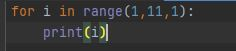
\includegraphics[width=0.5\textwidth]{figures/for1to10}%
	\hspace*{3mm}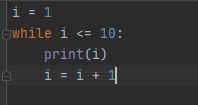
\includegraphics[width=0.5\textwidth]{figures/while1to10}
\end{figure}

\begin{itemize}
	\item recall: \texttt{range(1,11,1)} generates list \texttt{[1,2,3,4,5,6,7,8,9,10]} 
\end{itemize}

\end{frame}

%==============================================================

\begin{frame}[fragile]

\frametitle{ \texttt{for} vs.~\texttt{while}}

\begin{itemize}
	\item in \texttt{while} loop, counter \texttt{i} needs to be:
	\begin{itemize}
		\item \red{\emph{initialised}} before loop header
		\item \red{\emph{incremented}} in loop body
	\end{itemize}
	\item[]
	\item \texttt{for} loop does these two tasks automatically
	\item[]
	\item shorter \texttt{for} loop code here, but that does \emph{not} mean it's preferred in general
	\begin{itemize}
		\item \texttt{while} often more efficient
	\end{itemize}
	\item[]	
	\item which of \texttt{for} or \texttt{while} is ``best'' usually determined by problem at hand---both are useful!
\end{itemize}

\end{frame}

%==============================================================

\begin{frame}[fragile]

\frametitle{Example: Finding the maximum height}

\vspace*{-3mm}
\begin{figure}[ht]
	\centering
	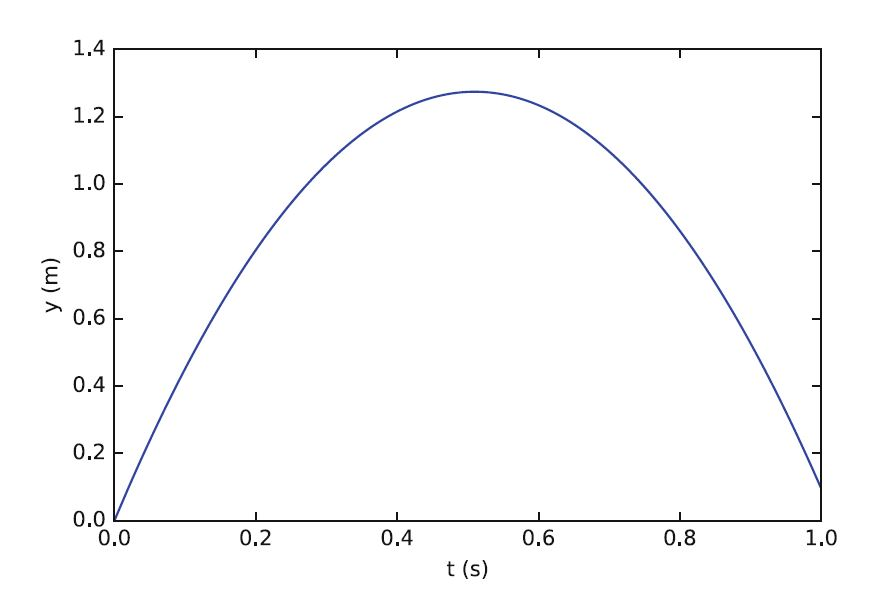
\includegraphics[width=0.6\textwidth]{figures/LLp20c}
\end{figure}
\vspace*{-3mm}
\begin{itemize}
	\item previously calculated height vs.\ time, and time of flight
	\item now calculate \textbf{maximum height} of ball
	\item will solve using \texttt{for} and \texttt{while} loops
\end{itemize}

\end{frame}

%==============================================================

\begin{frame}[fragile]

\frametitle{}

\begin{figure}[ht]
	\centering
	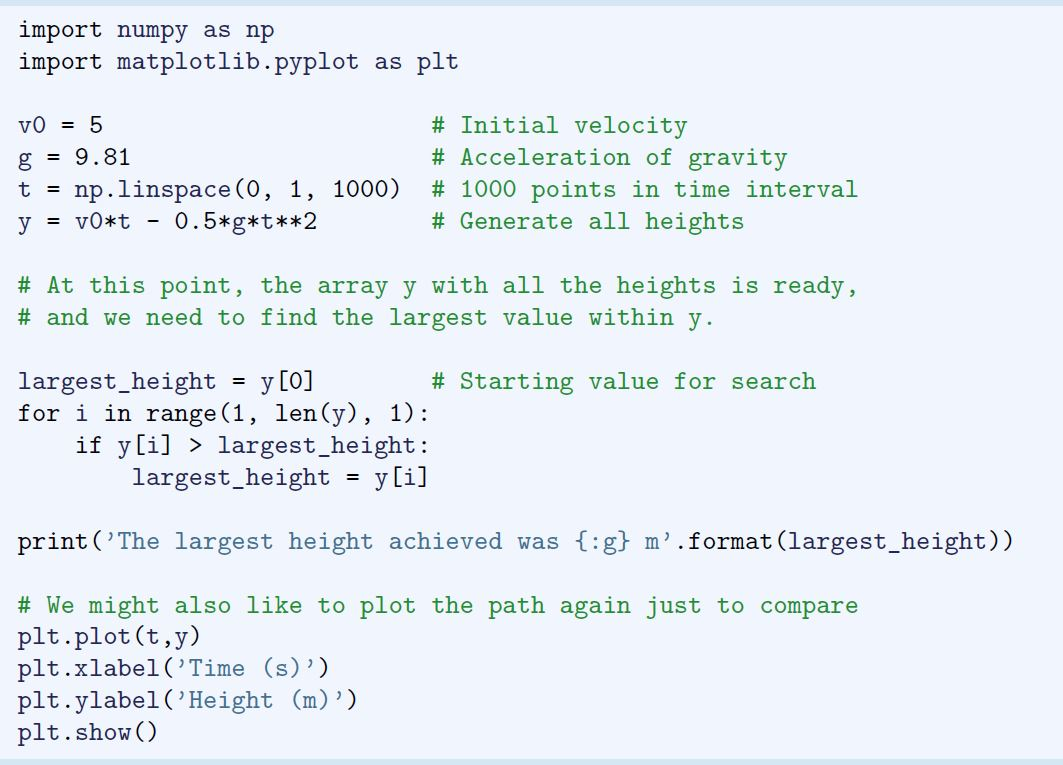
\includegraphics[width=0.9\textwidth]{figures/LLp71a}
\end{figure}
\vspace*{-3mm}
Python code:~\href{https://github.com/slgit/prog4comp_2/blob/master/py36-src/ball_max_height.py}{\texttt{ball\_max\_height.py}}

\end{frame}

%==============================================================

\begin{frame}[fragile]

\frametitle{Focus:~\texttt{for} loop to find max height}

Strategy:
\begin{itemize}
	\item compute array of ball heights, \texttt{y}
	\begin{itemize}
		\item values stored as \texttt{y[0], y[1], y[2], \ldots}
	\end{itemize}
	\item largest height initialised to \texttt{y[0]}
	\item work through remaining indices \texttt{i = 1,2,3,\ldots}
	\item each time \texttt{y[i]} is bigger than largest, it becomes the new largest
\end{itemize}

\begin{figure}[ht]
	\centering
	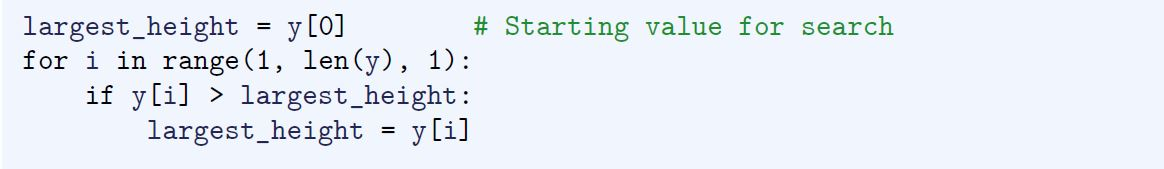
\includegraphics[width=\textwidth]{figures/LLp71b}
	
\includegraphics[width=\textwidth]{figures/LLp71c}
\end{figure}
\vspace*{-3mm}
\begin{itemize}
	\item live demo
\end{itemize}

\end{frame}

%==============================================================

\begin{frame}[fragile]

\frametitle{Focus:~\texttt{while} loop to find max height}

Strategy is to examine successive pairs of heights:
\begin{itemize}
	\item[]
	\begin{itemize}
		\item \texttt{y[0]} and \texttt{y[1]} 
		\item \texttt{y[1]} and \texttt{y[2]} 
		\item \texttt{y[2]} and \texttt{y[3]}
		\item $\cdots$
	\end{itemize}
	
	\item ball still rising when \texttt{y[i]} $<$ \texttt{y[i+1]}
	\item ball has reached maximum height when \\
	\item[] \texttt{y[i+1]} $\leq$ \texttt{y[i]}
	\begin{itemize}
		\item[] ie: when \texttt{y[i+1]} $>$ \texttt{y[i]} is \texttt{False}
	\end{itemize}
	\item report \texttt{y[i]} as maximum height
\end{itemize}

\begin{figure}[ht]
	\centering
	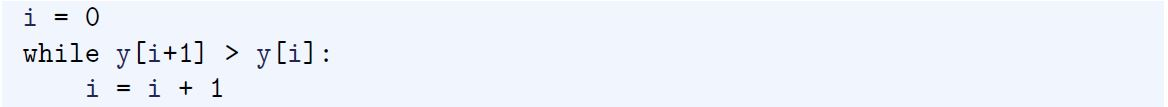
\includegraphics[width=\textwidth]{figures/LLp71d}
\end{figure}

\end{frame}

%==============================================================

\begin{frame}[fragile]

\frametitle{$2)$ Debugging strategies}

\begin{enumerate}
	\item running code by hand
	\begin{itemize}
		\item know what you expect your code to do
		\item use pen and paper to ``think like a computer''
		\item very easy to fool yourself with ``looks about right\ldots''
		\item use ``toy problems'': use tiny arrays, and values calculated at console
		\item near enough isn't good enough when debugging
	\end{itemize}
	
	\item don't guess, print!
	\begin{itemize}
		\item use temporary debug \texttt{print()} statements to check values and types of
		variables during loop iterations
	\end{itemize}
	\item take baby steps
		\begin{itemize}
			\item change one line at a time, then re-run code
			\item if interpreter generates an error, must have been the most recent change
		\end{itemize}
\end{enumerate}

\end{frame}

%==============================================================

\begin{frame}[fragile]

\frametitle{$3)$ Random numbers in Python}

\begin{itemize}
	\item Python provides ability to produce (apparently) random numbers
	\item[]
	\item referred to as \red{\emph{pseudo-random numbers}}
	\item[]
	\item these numbers are not \emph{truly} random
	\begin{itemize}
		\item produced in a complicated (but ``deterministic'' or predictable) way once a \red{\emph{seed}} has been set
	\end{itemize}	
	\item[]
	\item seed is a number which depends on the current time
		
\end{itemize}

\end{frame}

%==============================================================

\begin{frame}[fragile]

\frametitle{Drawing \textbf{one} random number at a time}

\begin{figure}[ht]
	\centering
	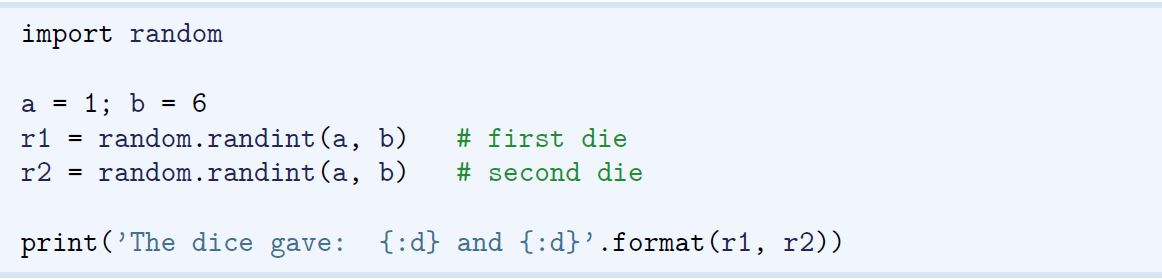
\includegraphics[width=\textwidth]{figures/LLp54}
\end{figure}

Python code:~\href{https://github.com/slgit/prog4comp_2/blob/master/py36-src/throw_2_dice.py}{\texttt{throw\_2\_dice.py}}

\begin{itemize}
	\item function \texttt{randint(a,b)}
	\begin{itemize}
		\item available from imported module \texttt{random} %, part of the standard Python library
		\item returns a pseudo-random \emph{integer} in the range $[a,b]$ where $a \leq b$
	\end{itemize}
\end{itemize}

\end{frame}

%==============================================================

\begin{frame}[fragile]

\frametitle{Fixing the seed}

\begin{itemize}
	\item when debugging programs that involve pseudo-random numbers, often helps to \red{\emph{fix the seed}}
	\item[]
	\item ensures that \emph{identical sequence of numbers will be generated} each time code is run
	\begin{itemize}
		\item hence results are \emph{repeatable}
	\end{itemize}
	\item[]
	\item tell Python what seed should be using \texttt{random.seed} function
	\item[]
	\item \textbf{Example:} \texttt{random.seed(10)} and run Python code:~\href{https://github.com/slgit/prog4comp_2/blob/master/py36-src/throw_2_dice.py}{\texttt{throw\_2\_dice.py}}
\end{itemize}

\end{frame}

%==============================================================

\begin{frame}[fragile]

\frametitle{Two functions: \texttt{random} and \texttt{uniform}}

\begin{itemize}
	\item both \texttt{random} and \texttt{uniform} return a floating point number from an interval where each number has \emph{equal probability} of being drawn
	\begin{itemize}
		\item random number drawn from \red{\emph{uniform}} probability distribution
		\item Note: \texttt{random} function in \texttt{random} module
	\end{itemize}
	\item[]
	\item \texttt{random}
	\begin{itemize}
		\item draw from interval $[0, 1)$
%		\item 0 is included, but 1 is not
	\end{itemize}
	
	\item[]
	\item \texttt{uniform}
	\begin{itemize}
		\item draw from interval $[a, b]$
	\end{itemize}

%	\item text doesn't mention Gaussian (normal) random numbers
\end{itemize}

\end{frame}

%==============================================================

\begin{frame}[fragile]

\frametitle{Live demo:~\texttt{random} and \texttt{uniform}}

\begin{figure}[ht]
	\centering
	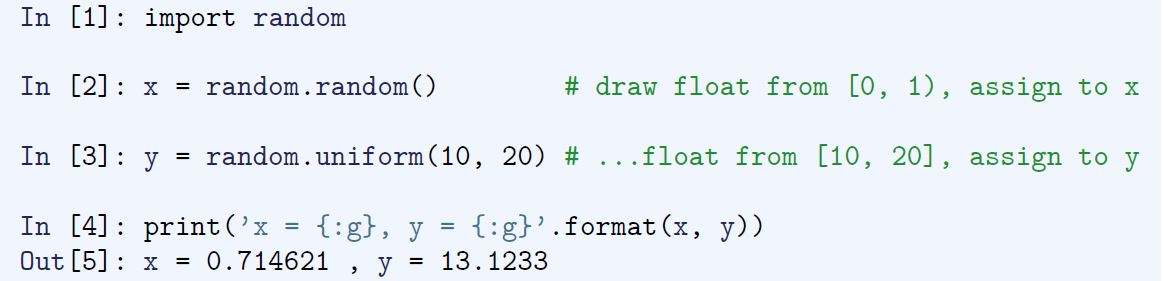
\includegraphics[width=\textwidth]{figures/LLp55a}
\end{figure}

\end{frame}

%==============================================================

\begin{frame}[fragile]

\frametitle{Drawing \textbf{many} random numbers at a time}

\begin{itemize}
	\item three random number generators seen so far
	\begin{itemize}
		\item each generates just \emph{one} random number at a time
	\end{itemize}
	\item[]
	\item to generate an \emph{array} of random numbers\ldots
	\item[] \ldots could use a loop \& generate one random number in each iteration
	\item[]
	\item better (faster) solution: use \texttt{random} module in \texttt{numpy} library

\end{itemize}

\end{frame}

%==============================================================

\begin{frame}[fragile]

\frametitle{Live demo: random numbers from \texttt{numpy} library}

\textbf{Example:} \texttt{np.random.randint}

\begin{itemize}
	\item[]
	\begin{itemize}
		\item \texttt{numpy} library / \texttt{random} module / \texttt{randint} function
		\item \texttt{randint(a,b,n)} generates $n$ integers from $[a,b)$
	\end{itemize}
\end{itemize}

\begin{figure}[ht]
	\centering
	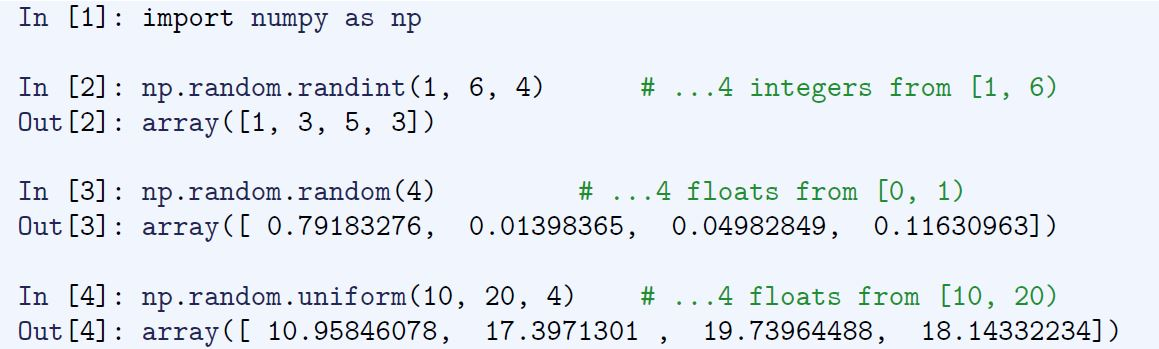
\includegraphics[width=\textwidth]{figures/LLp55b}
\end{figure}

\begin{itemize}
	\item live demo, also fix seed:~\texttt{np.random.seed(10)}
\end{itemize}

\end{frame}

%==============================================================

\begin{frame}[fragile]

\frametitle{Lecture summary}
\begin{itemize}
	\item Iteration again
	\begin{itemize}
		\item \texttt{for} vs.~\texttt{while}
	\end{itemize}

	\item[]
	
	\item Debugging strategies
	\begin{itemize}
		\item running code by hand
		\item don't guess, print!
		\item take baby steps
	\end{itemize}

	\item[]
	
	\item Random numbers
		\begin{itemize}
			\item random module---random numbers one at a time %: \texttt{randint}, \texttt{random} and \texttt{uniform}
			\item random module in \texttt{numpy} library---arrays of random numbers % :~\texttt{randint}, \texttt{random} and \texttt{uniform}
		\end{itemize}
		
\end{itemize}

\end{frame}

\end{document}